\chapter{Projeto Conceitual do Produto}

\section{Características gerais}

\textcolor{red}{Descrever produto de forma geral. Apresentar itens teóricos sobre o projeto a serem aprofundados ou detalhados oportunamente.}

\textcolor{red}{Apresentar e explicar a Estrutura Analítica do Projeto (EAP), tomando cuidado com a legibilidade da imagem. Se necessário, coloque a EAP dentro do comando ``\textsf{\textbackslash begin\{landscape\} \textbackslash end\{landscape\}}'' para que ela seja apresentada em uma página deitada.}

\section{Estrutura}

\textcolor{red}{Apresentar desenho em CAD, indicar dimensões por lado/aresta/cota, indicar materiais utilizados e explicar o desenho e as decisões de projeto.}

\section{Descrição de \textit{hardware}}

\textcolor{red}{A descrição de \textit{hardware} no documento deve permitir que outras pessoas repliquem o produto proposto neste documento. Para isso, deve-se explicar de forma textual os principais sub-sistemas e as escolhas de projeto, além de indicar:}

\begin{itemize}
    \item \textcolor{red}{ O diagrama de blocos \cite{blockdiagram}, que oferece uma visão geral do hardware, com as principais partes do sistema e as ligações entre elas.}
    %\item A lista de materiais \cite{bom}, que facilita a montagem do sistema, indicando tudo que deve ser adquirido. Aproveitem a lista de materiais para apresentarem o orçamento dos mesmos.
    \item \textcolor{red}{ O esquemático \cite{esquematico}, que mostra as conexões elétricas entre os componentes. Deve-se indicar os componentes por nomes e símbolos, e as conexões entre eles, incluindo a pinagem dos componentes. Se o esquemático ficar muito grande, pode-se separa-lo em vários esquemáticos. A ligação em \textit{protoboard} não é considerada um esquemático adequado.}
\end{itemize}

\textcolor{red}{A Fig. \ref{fig:diagrama_blocos_e_esquematico} apresenta o diagrama de blocos e o esquemático de um circuito conversor de corrente alternada para corrente direta, a título de exemplo. Repare que o diagrama de blocos indica os subsistemas do circuito completo apresentado no esquemático.
% Comecem com o diagrama de blocos, que é mais genérico, e depois indiquem os detalhes com a lista de materiais e os esquemáticos.
}

\begin{figure}
    \centering
    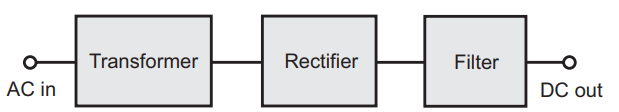
\includegraphics[width=0.5\linewidth]{figuras/Exemplo-diagrama-de-blocos.png}
    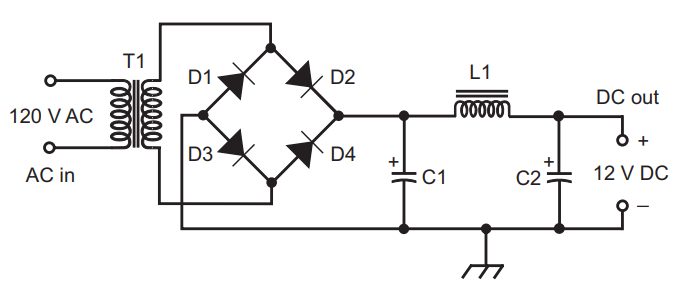
\includegraphics[width=0.5\linewidth]{figuras/Esquematico.png}
    \caption{\textcolor{red}{Diagrama de blocos e esquemático de um circuito conversor de corrente alternada para corrente direta. Extraído de \cite{block_n_schematic}.}}
    \label{fig:diagrama_blocos_e_esquematico}
\end{figure}

\section{Análise de consumo energético}

O subgrupo de Energia é responsável por garantir a alimentação elétrica do micromouse. O trabalho foca em fornecer energia estável para os motores, sensores e o microcontrolador ESP32.

O grupo realiza o cálculo do gasto energético de cada componente, seleciona a fonte de alimentação (bateria ou pilhas) e projeta os circuitos de regulação de tensão. Além disso, o sistema deve permitir o monitoramento do nível de carga para que o dado seja enviado via telemetria.

\subsection{Frentes de trabalho}
As atividades estão divididas em:
\begin{itemize}
    \item \textbf{Dimensionamento:} Cálculo da corrente e energia total (Joules e Watt-hora).
    \item \textbf{Regulação de Tensão:} Conversão da tensão da fonte (7.2V) para os níveis de operação (5V e 3.3V).
    \item \textbf{Proteção e Segurança:} Gestão térmica e prevenção de danos por picos de corrente.
    \item \textbf{Monitoramento:} Implementação de divisor de tensão para leitura analógica da carga.
\end{itemize}

\subsection{Identificação dos subsistemas elétricos}
Após consulta das datasheets de cada um dos componentes, foram obtidos os seguintes dados de tensão e de corrente estimadas, organizados na seguinte tabela:

\begin{table}[h]
\centering
\renewcommand{\arraystretch}{1.3} % Aumenta um pouco o espaçamento das linhas para melhor leitura
\resizebox{\textwidth}{!}{%
\begin{tabular}{|l|c|c|}
\hline
\textbf{Componente} & \textbf{Tensão de Operação (V)} & \textbf{Corrente Estimada (mA)} \\ \hline
ESP32 (Wi-Fi e Bluetooth)       & 3.3 - 3.6     & 500           \\ \hline
02 Motores DC (Redução 48:1)    & 3.0 - 6.0     & 800-1000      \\ \hline
Driver Duplo Ponte H (DRV8833)  & 2.7 - 10.8    & 3             \\ \hline
Sensor IR (KY-032)              & 3.3 - 5.0     & 20            \\ \hline
Sensor Óptico ToF (VL53L0X)     & 3.3 - 5.0     & 20            \\ \hline
IMU (MPU6050 GY521)             & 3.3 - 5.0     & 5             \\ \hline
Mini Protoboard (170 pontos)    & -             & 0             \\ \hline\hline
\textbf{Total Necessário} & \textbf{5.0 (Fonte Principal)} & \textbf{$\approx$ 1050} \\ \hline
\end{tabular}}
\caption{Dimensionamento de Tensão e Corrente dos Componentes do Robô}
\label{tab:dimensionamento_energia}
\end{table}

\subsection{Cálculo da energia consumida por componente}
Para o cálculo da energia consumida por componente, foi utilizada a fórmula:
\[
    \ E = V (Volts) \cdot I (A) \cdot \Delta t (s)      [J]
\]

\begin{table}[h!]
\centering
\renewcommand{\arraystretch}{1.3}
\resizebox{\textwidth}{!}{%
\begin{tabular}{|l|c|c|c|c|}
\hline
\textbf{Componente} & \textbf{V (Volts)} & \textbf{I (Ampères)} & \textbf{t (Segundos)} & \textbf{E (Joules)} \\ \hline
ESP32 (Wi-Fi e Bluetooth)           & 3.3 & 0.500 & 1800 & 2970.0   \\ \hline
02 Motores DC (Redução 48:1)        & 5.0 & 1.000 & 1800 & 9000.0   \\ \hline
Driver Duplo Ponte H (DRV8833)      & 5.0 & 0.003 & 1800 & 27.0     \\ \hline
Sensor IR (KY-032)                  & 3.3 & 0.020 & 1800 & 118.8    \\ \hline
Sensor Óptico ToF (VL53L0X)         & 3.3 & 0.020 & 1800 & 118.8    \\ \hline
IMU (MPU6050 GY521)                 & 3.3 & 0.005 & 1800 & 29.7     \\ \hline\hline
\textbf{Total Estimado} & \textbf{-} & \textbf{-} & \textbf{1800} & \textbf{12264.3} \\ \hline
\end{tabular}}
\caption{Cálculo da Energia Consumida (Autonomia de 30 minutos com valores de pico)}
\label{tab:energia_componentes_pico}
\end{table}

\subsection{Escolha da fonte de alimentação}
\subsection*{Conversão para Watt-hora}
A partir do cálculo de consumo total do sistema para uma autonomia de aproximadamente 30 minutos, obtivemos uma energia consumida de 8700,3 J. Utilizando a relação de conversão de que 1 Wh=3600 J, temos:
\[
    \frac{12364,3 [J]}{3600} \approx 3,43 Wh
\]
\subsection*{Justificativas e Aplicação da Margem de Segurança}
É considerada boa prática utilizar uma margem de segurança de cerca de 20\% a 30\%. Essa margem é essencial por três motivos:
\begin{enumerate}
    \item \textbf{Corrente de Stall:} No momento em que o robô liga e arranca ou bate em uma parede e fica preso, os motores exigirão uma corrente maior.
    \item \textbf{Perdas térmicas e degradação da tensão:} À medida que a bateria descarrega, a tensão da mesma tende a cair, de modo a exigir mais corrente para manter a mesma potência, e também, o regulador de tensão interno da ESP32 dissipa parte da energia em forma de calor, pode ser uma quantidade insignificativa, porém, como as opções de bateria que serão apresentadas posteriormente estão na faixa mais baixa do limiar mínimo necessário, o grupo acha válido considerar uma margem de segurança mais generosa.
\end{enumerate}

Adotando uma margem de 20\%, o requisito de energia final passa a ser:
\[
    E = 3,43 \times 1,20 \approx 4,12 Wh
\]
 
Para suprir a demanda energética do projeto com margem de segurança (4,79 Wh), optou-se pela opção de alimentação por um banco de 6 pilhas AA recarregáveis (NiMH). Este arranjo fornece uma tensão nominal de 7.2V e capacidade média de 2000 mAh (totalizando cerca de 14,4 Wh), atendendo aos requisitos de energia e mantendo a estabilidade da tensão frente aos picos de corrente de tração. Outra opção viável seria a adaptação de um powerbank de 5V/2A, que já teria um circuito de estabilização de tensão.

\section{Descrição de \textit{software}}

O subgrupo de software é responsável por dois componentes principais e interdependentes: o \textbf{software embarcado}, executado no microcontrolador ESP32 do robô, e o \textbf{sistema web de telemetria}, responsável pela visualização e armazenamento dos dados de cada corrida.

\begin{center}
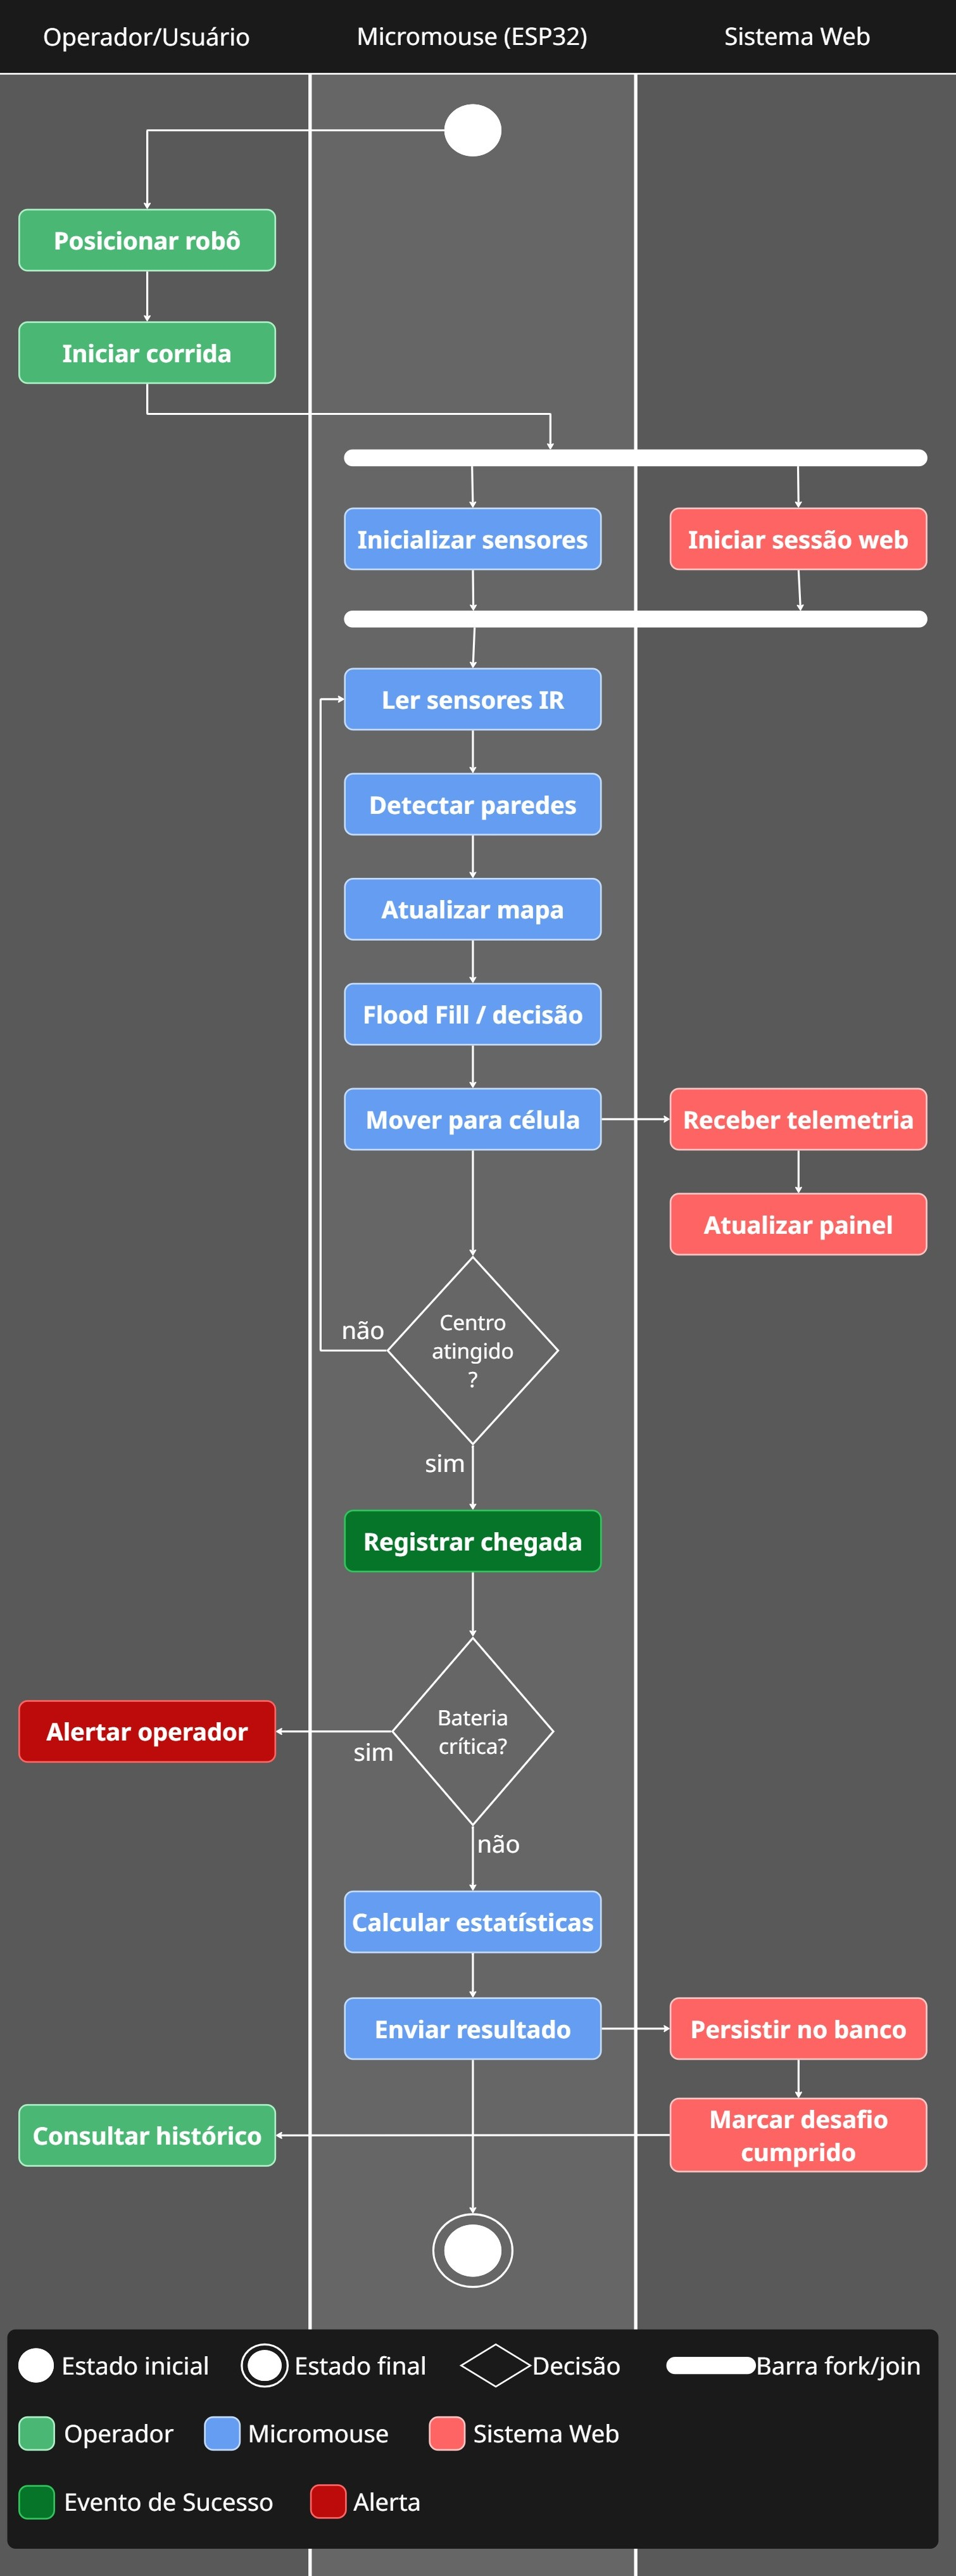
\includegraphics[
    width=0.95\textwidth,
    height=0.8\textheight,
    keepaspectratio
]{figuras/diagrama_atividades_uml.jpg}

\captionof{figure}{Diagrama de Atividades UML.}
\label{fig:diagramauml_fig}
\end{center}

O fluxo está dividido em três raias (\textit{swimlanes}): Operador/Usuário, Micromouse (ESP32) e Sistema Web. O processo começa com o operador posicionando o robô e disparando o início da corrida. A partir daí, uma barra de bifurcação (\textit{fork}) representa o paralelismo: o ESP32 inicializa seus sensores ao mesmo tempo que o sistema web abre a sessão de telemetria. Uma barra de junção (\textit{join}) sincroniza as duas trilhas antes do loop principal.

O ciclo de exploração repete: leitura dos sensores IR $\rightarrow$ detecção de paredes $\rightarrow$ atualização do mapa $\rightarrow$ algoritmo Flood Fill $\rightarrow$ movimentação. A cada passo, a telemetria é enviada ao sistema web em paralelo (velocidade, trajeto, bateria). Dois nós de decisão controlam a saída do loop: ``centro atingido?'' e ``bateria crítica?''. O alerta de bateria deriva para o operador e reintegra o fluxo. Ao atingir o centro, o robô calcula as estatísticas finais, envia ao sistema web, que persiste no banco e marca o campo ``Desafio cumprido''.

\subsubsection*{Backlog do Produto}
 
O backlog foi elaborado com base nos requisitos funcionais (RF) e não funcionais (RNF) definidos no Capítulo 2, priorizados pela classificação MoSCoW.

\paragraph{Histórias de Usuário (Requisitos Funcionais)}
 
\begin{itemize}

    \item \textbf{HU01 – Resolução autônoma do labirinto} [\textit{Must have}]\\
    \textit{Eu, como} avaliador do projeto, \textit{quero} que o sistema permita visualizar e validar a execução da resolução autônoma de labirintos de tamanhos 4×4, 8×8 e 16×16, \textit{para} verificar a capacidade de navegação sem intervenção humana.\\
    \textbf{Critérios de aceitação:} o robô deve atingir o centro do labirinto sem tocar nas paredes e sem qualquer interação externa durante a tentativa.

    \begin{center}
    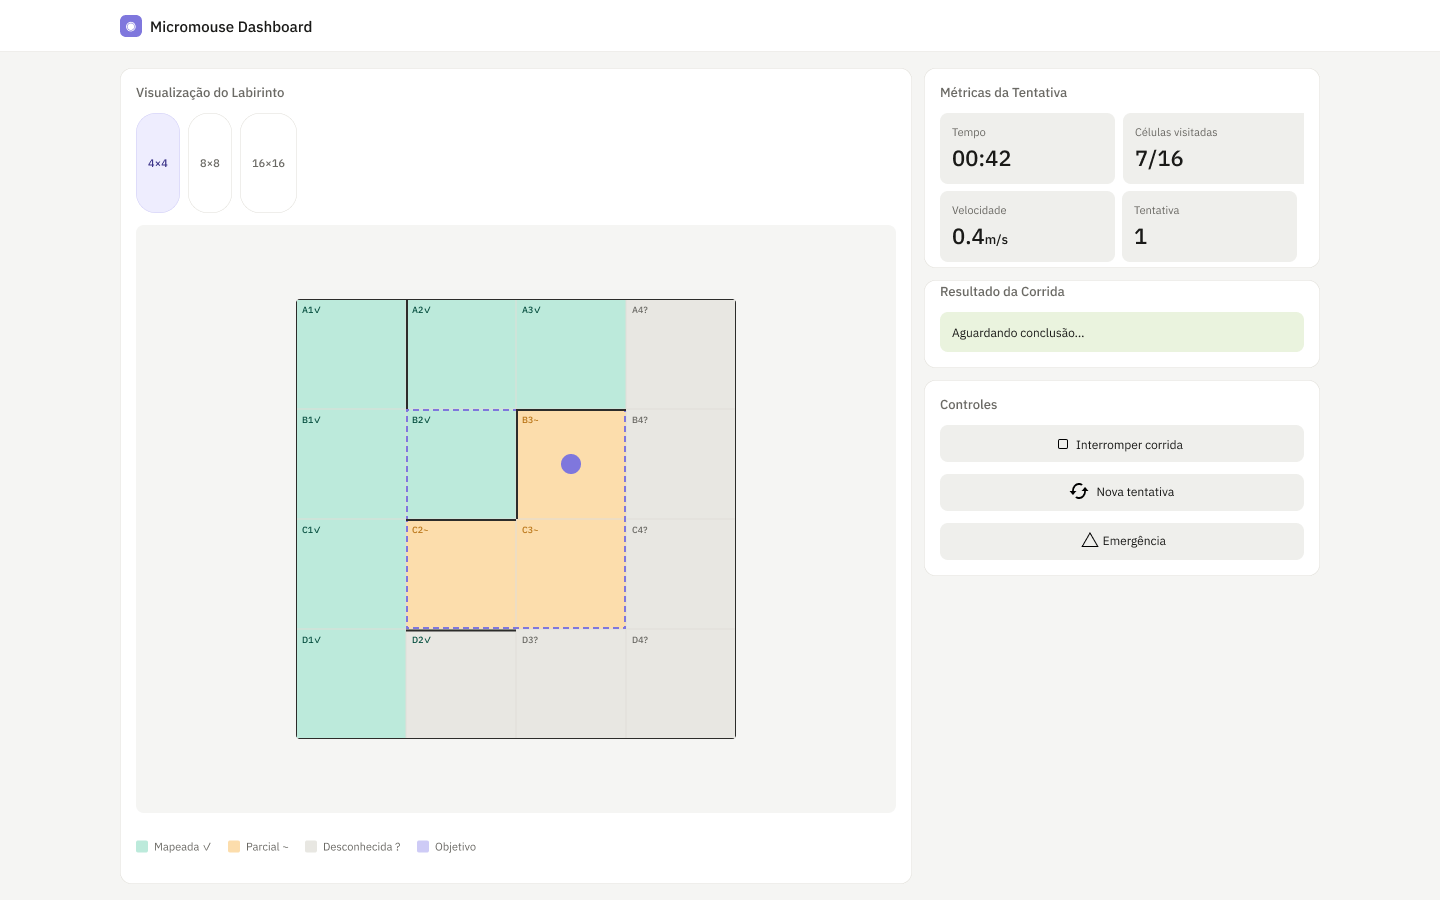
\includegraphics[
        width=0.95\textwidth,
        height=0.8\textheight,
        keepaspectratio
    ]{figuras/HU01–Execução autônoma.png}

    \captionof{figure}{Protótipo da HU01.}
    \label{fig:execucaoautonoma_fig}
    \end{center}
 
    \item \textbf{HU02 – Mapeamento incremental do labirinto} [\textit{Must have}]\\
    \textit{Eu, como} desenvolvedor do sistema embarcado, \textit{quero} que o robô detecte e registre paredes à medida que explora, \textit{para} construir o mapa do labirinto em tempo de execução.\\
    \textbf{Critérios de aceitação:} após a primeira corrida em um labirinto 4×4, ao menos 80\% das células devem ter sido corretamente mapeadas.

    \begin{center}
    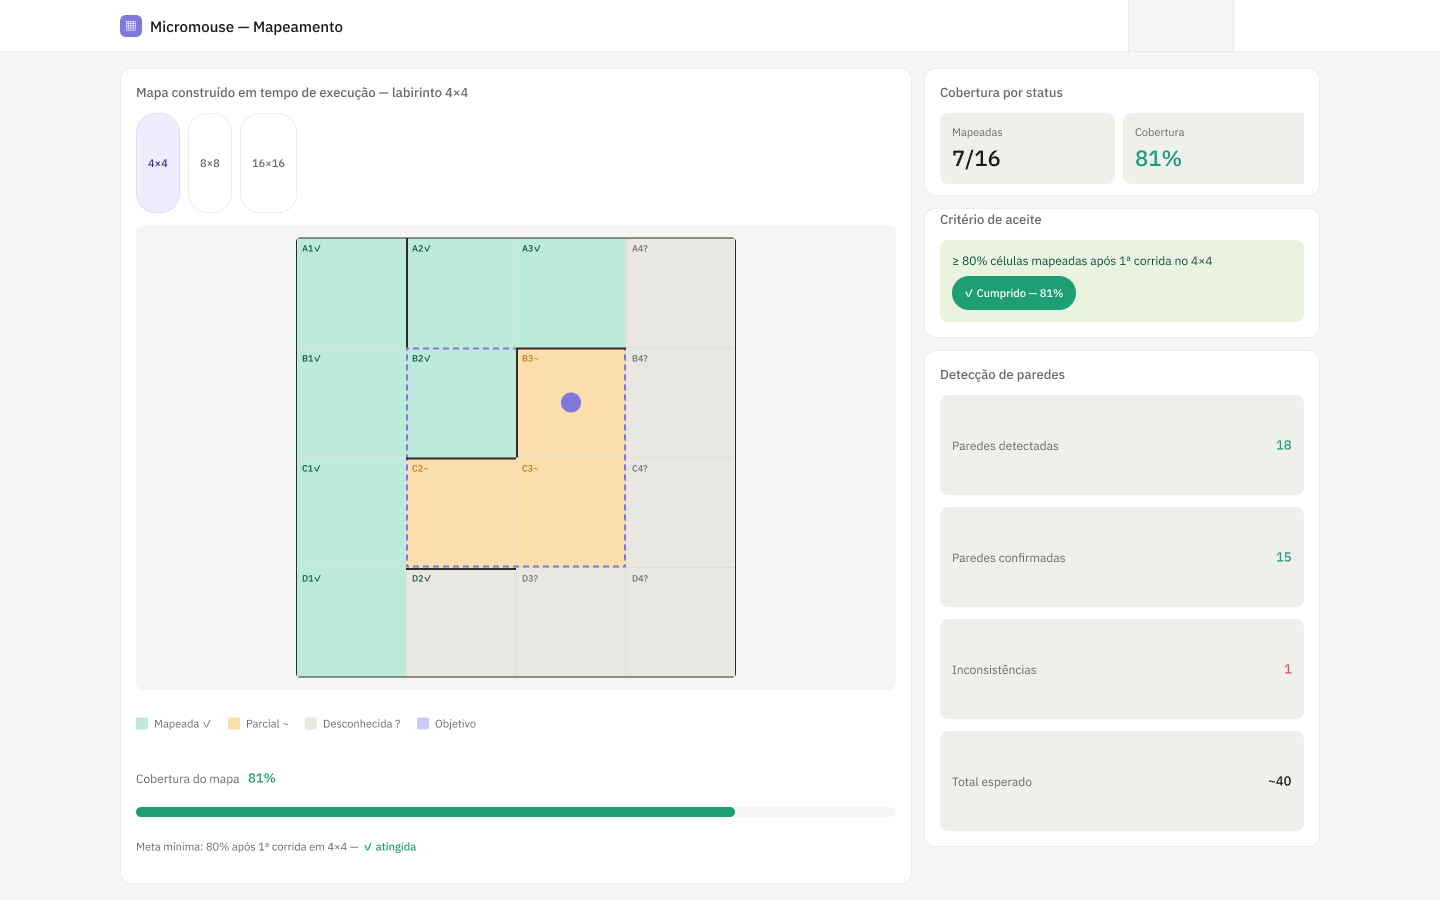
\includegraphics[
        width=0.95\textwidth,
        height=0.8\textheight,
        keepaspectratio
    ]{figuras/HU02–Mapeamento incremental.png}

    \captionof{figure}{Protótipo da HU02.}
    \label{fig:mapeamento_fig}
    \end{center}

    \item \textbf{HU03 – Telemetria em tempo real} [\textit{Must have}]\\
    \textit{Eu, como} observador da corrida, \textit{quero} visualizar no painel web o trajeto percorrido, o tempo, a velocidade média e o nível de bateria em tempo real, \textit{para} acompanhar o desempenho do robô durante a tentativa.\\
    \textbf{Critérios de aceitação:} os dados devem ser atualizados no painel com latência máxima estipulada pela equipe, sem gargalos visuais perceptíveis.

    \begin{center}
    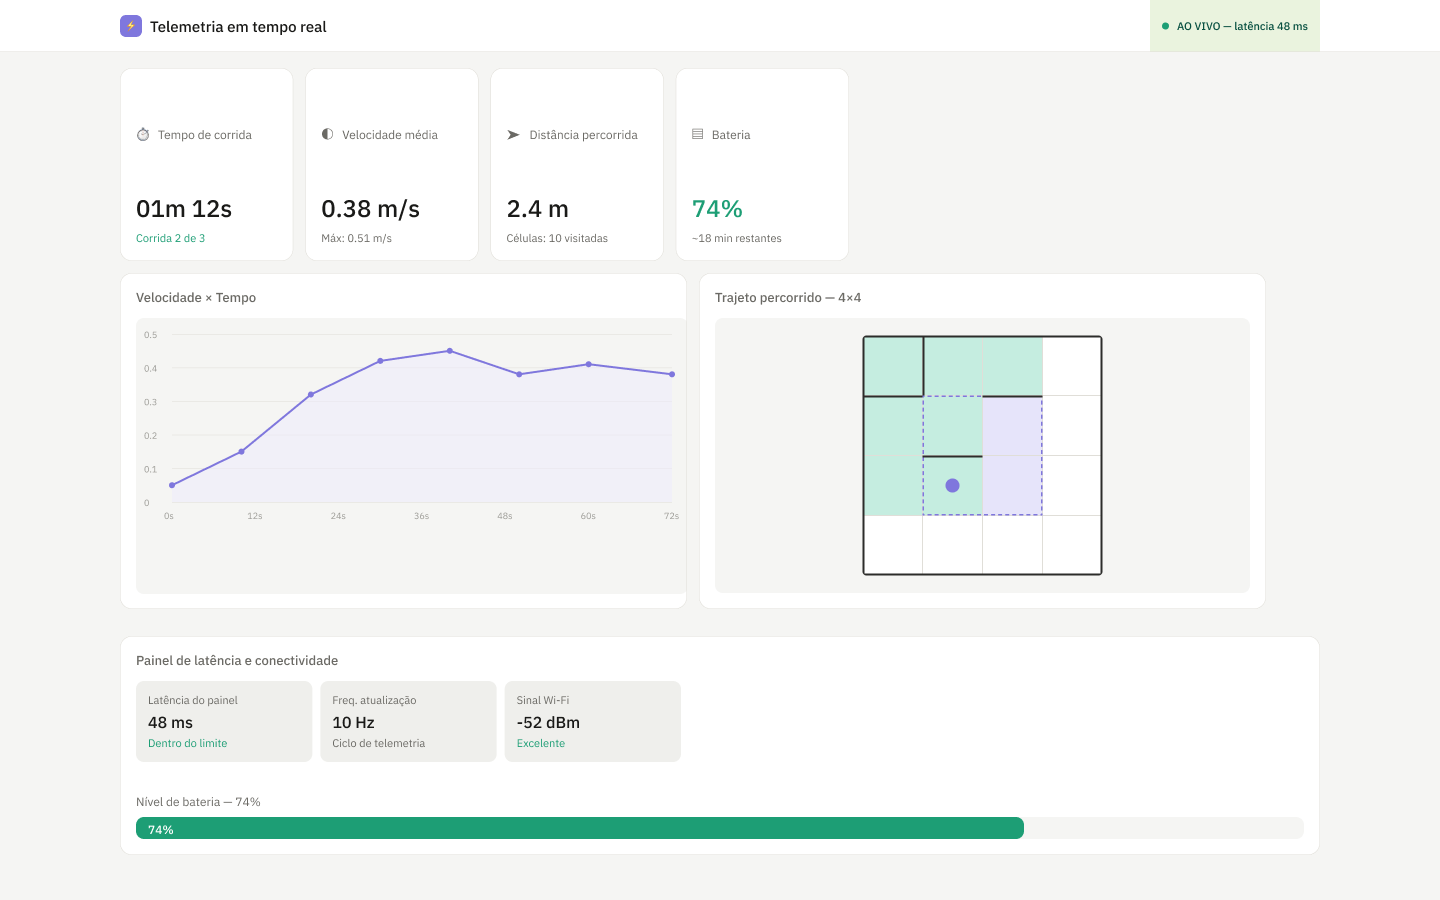
\includegraphics[
        width=0.95\textwidth,
        height=0.8\textheight,
        keepaspectratio
    ]{figuras/HU03–Telemetria em tempo real.png}

    \captionof{figure}{Protótipo da HU03.}
    \label{fig:telemetria_fig}
    \end{center}
 
    \item \textbf{HU04 – Persistência e consulta de histórico} [\textit{Must have}]\\
    \textit{Eu, como} professor avaliador, \textit{quero} consultar os resultados de corridas anteriores filtradas por labirinto, \textit{para} comparar o desempenho do robô ao longo do projeto.\\
    \textbf{Critérios de aceitação:} os dados finais de cada corrida concluída devem ser gravados no banco de dados e recuperáveis pela interface de histórico com filtro por tamanho de labirinto.

    \begin{center}
    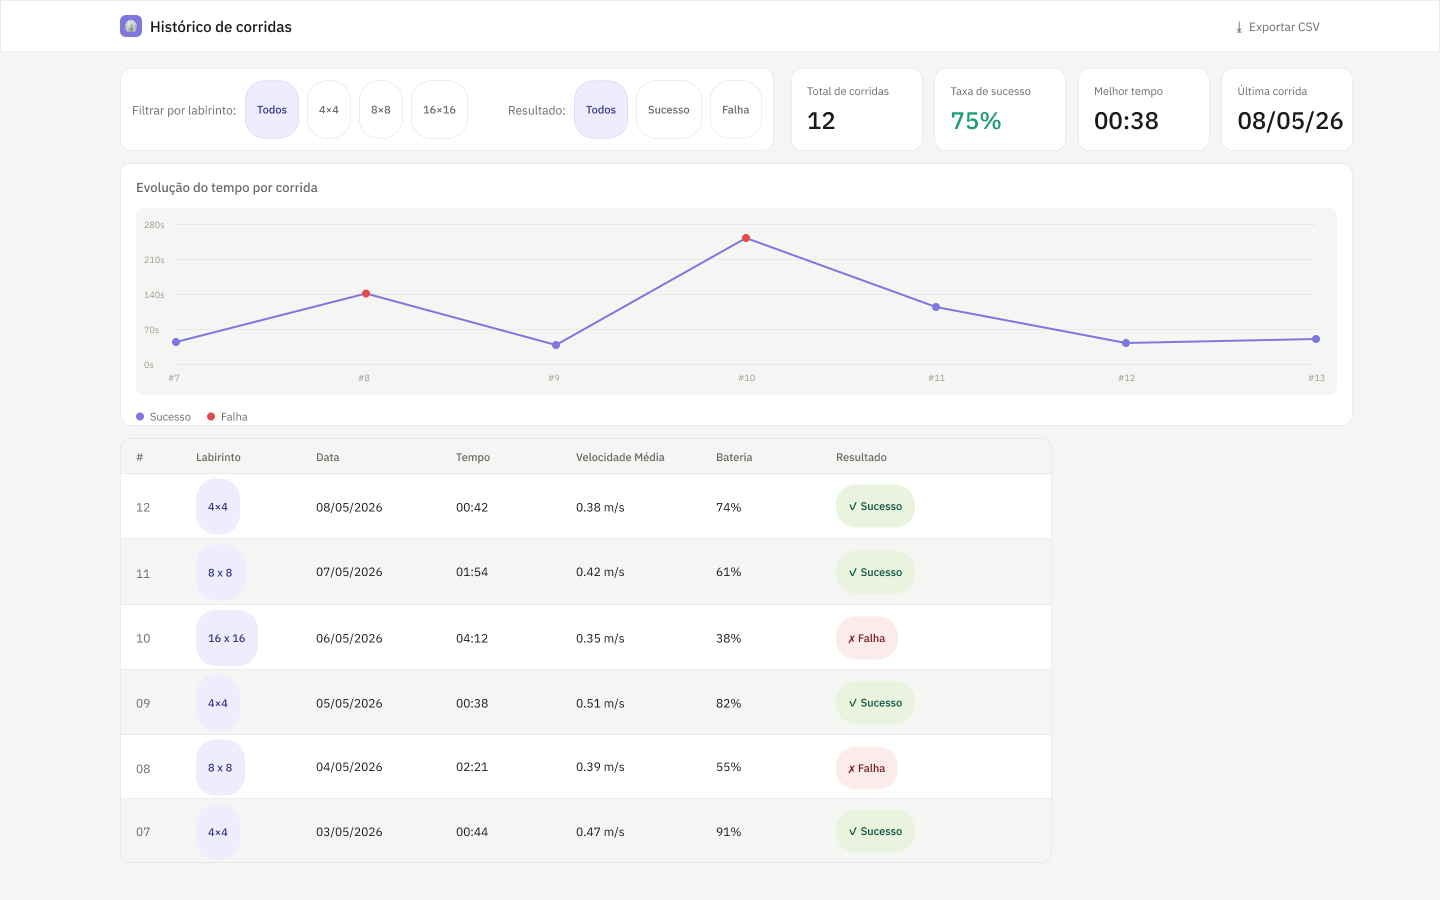
\includegraphics[
        width=0.95\textwidth,
        height=0.8\textheight,
        keepaspectratio
    ]{figuras/HU04–Histórico de corridas.png}

    \captionof{figure}{Protótipo da HU04.}
    \label{fig:historicocorridas_fig}
    \end{center}
 
    \item \textbf{HU05 – Monitoramento de bateria} [\textit{Should have}]\\
    \textit{Eu, como} operador do robô, \textit{quero} visualizar no painel web o nível percentual de carga da bateria enviado pelo sistema embarcado, \textit{para} evitar interrupções inesperadas durante as corridas.\\
    \textbf{Critérios de aceitação:} o nível de bateria deve ser lido via divisor de tensão pelo ESP32 e exibido no painel web com atualização a cada ciclo de telemetria.

    \begin{center}
    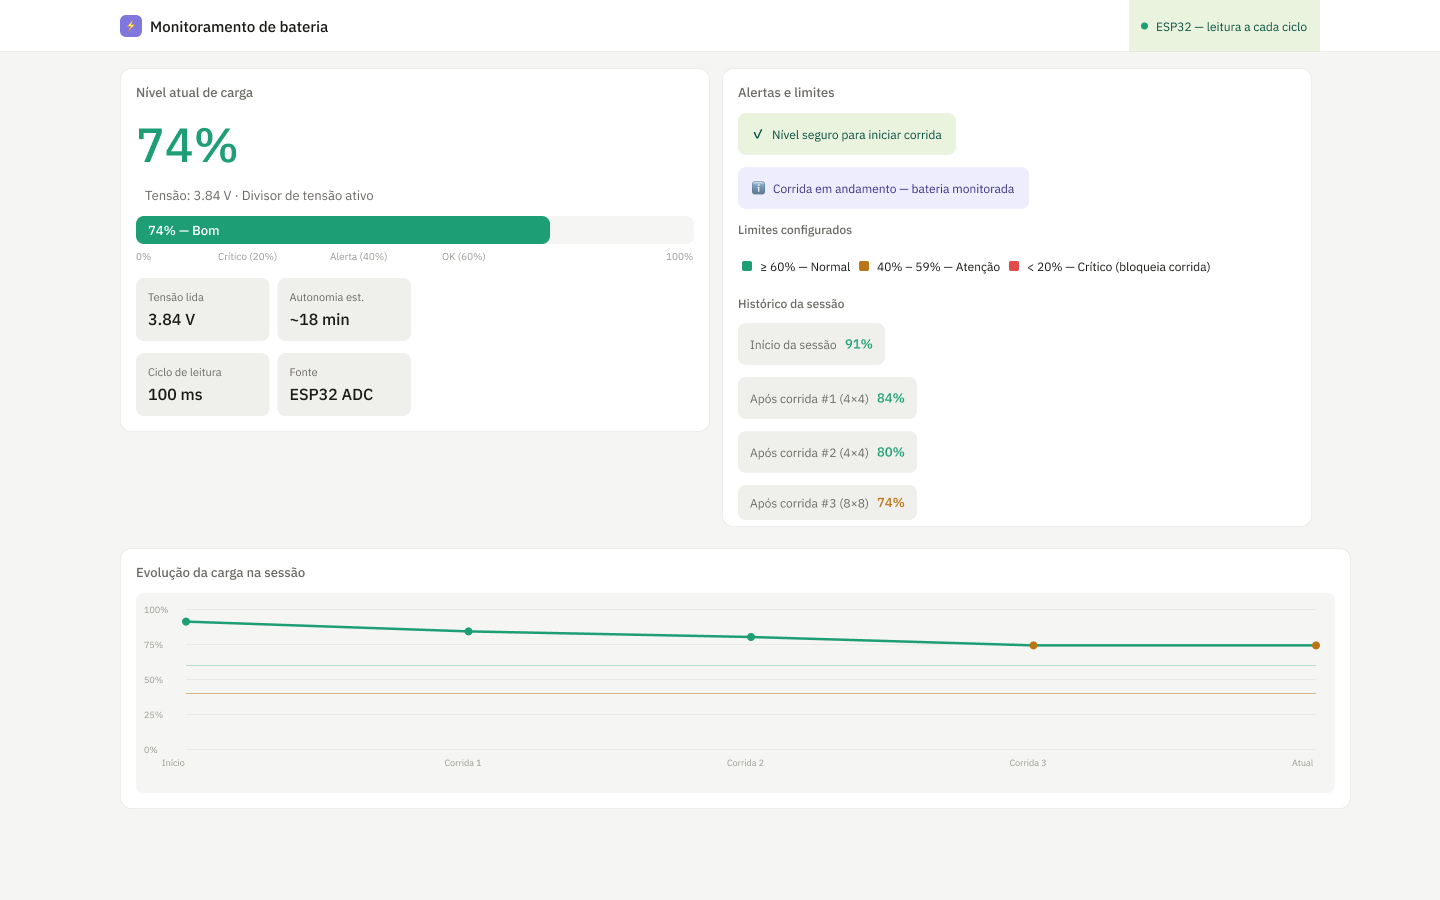
\includegraphics[
        width=0.95\textwidth,
        height=0.8\textheight,
        keepaspectratio
    ]{figuras/HU05–Monitoramento de bateria.png}

    \captionof{figure}{Protótipo da HU05.}
    \label{fig:monitoramentobateria_fig}
    \end{center}
 
    \item \textbf{HU06 – Indicador de desafio cumprido} [\textit{Could have}]\\
    \textit{Eu, como} usuário do sistema web, \textit{quero} visualizar se o desafio foi cumprido (Sim/Não) ao término de cada corrida, \textit{para} identificar rapidamente o resultado no histórico.\\
    \textbf{Critérios de aceitação:} ao final de cada corrida, o campo ``Desafio cumprido'' deve ser preenchido automaticamente com base na detecção da chegada ao centro.

    \begin{center}
    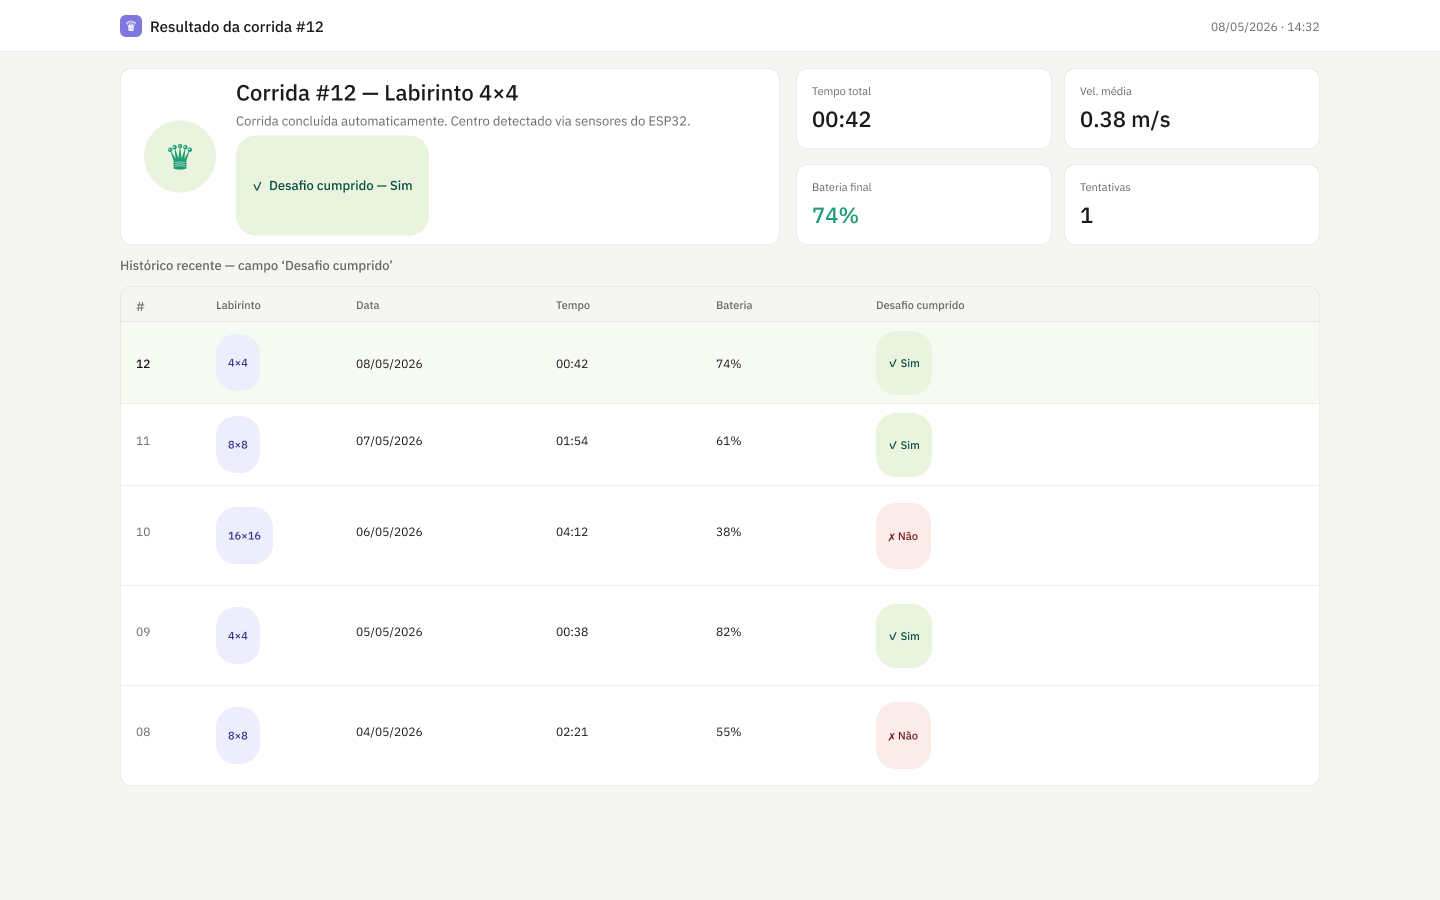
\includegraphics[
        width=0.95\textwidth,
        height=0.8\textheight,
        keepaspectratio
    ]{figuras/HU06–Desafio cumprido.png}

    \captionof{figure}{Protótipo da HU06.}
    \label{fig:desafiocumprido_fig}
    \end{center}
 
\end{itemize}
 
\paragraph{Requisitos Não Funcionais}
 
\begin{itemize}
    \item \textbf{RNF01} [\textit{Must have}] – O código-fonte embarcado e a memória do labirinto não podem ser alterados durante a execução de uma tentativa na pista.
    \item \textbf{RNF02} [\textit{Must have}] – O sistema embarcado deve operar com o microcontrolador ESP32 como unidade central de processamento.
    \item \textbf{RNF03} [\textit{Must have}] – A latência da telemetria deve ser estipulada e estabilizada de modo que a atualização do painel ocorra sem gargalos perceptíveis em tempo real.
    \item \textbf{RNF04} [\textit{Must have}] – Nenhuma solução de software pronta pode substituir o desenvolvimento próprio dos módulos exigidos pelo escopo.
    \item \textbf{RNF05} [\textit{Should have}] – Cada \textit{issue} no GitHub deve ter no máximo dois responsáveis, garantindo rastreabilidade individual das contribuições.
    \item \textbf{RNF06} [\textit{Should have}] – Ferramentas de inteligência artificial generativa não podem ser utilizadas nas atividades avaliativas do subgrupo.
\end{itemize}

\paragraph{Casos de Uso}

\begin{center}
\begin{longtable}{|l|c|p{5.5cm}|p{3cm}|c|}
\caption{Casos de uso funcionais -- Backlog do Micromouse.} \label{tab:backlog-uc} \\

\hline
\textbf{ID} & \textbf{HU orig.} & \textbf{Caso de uso} & \textbf{Atores} & \textbf{Prioridade} \\ \hline
\endfirsthead

\multicolumn{5}{c}%
{{\bfseries Tabela \thetable{} -- continuação da página anterior}} \\
\hline
\textbf{ID} & \textbf{HU orig.} & \textbf{Caso de uso} & \textbf{Atores} & \textbf{Prioridade} \\ \hline
\endhead

\hline \multicolumn{5}{|r|}{{Continua na próxima página...}} \\ \hline
\endfoot

\hline
\endlastfoot

\multicolumn{5}{|l|}{\textit{Módulo embarcado -- ESP32}} \\ \hline

UC01 & HU01 & Resolver labirinto autonomamente & Micromouse & Must have \\ \hline
UC02 & HU02 & Mapear labirinto incrementalmente & Micromouse & Must have \\ \hline
UC03 & HU02 & Ler sensores IR de distância & Micromouse & Must have \\ \hline
UC04 & HU01 & Executar algoritmo de navegação & Micromouse & Must have \\ \hline
UC05 & HU05 & Monitorar nível de bateria & Micromouse & Should have \\ \hline
UC06 & HU03 & Transmitir dados de telemetria & Micromouse & Must have \\ \hline
UC07 & HU01 & Registrar chegada ao centro & Micromouse & Must have \\ \hline
UC08 & HU01 & Calcular estatísticas finais & Micromouse & Must have \\ \hline

\multicolumn{5}{|l|}{\textit{Módulo web -- painel de telemetria}} \\ \hline

UC09 & HU03 & Visualizar telemetria & Operador, Avaliador & Must have \\ \hline
UC10 & HU05 & Exibir nível de bateria no painel & Operador & Should have \\ \hline
UC11 & HU04 & Consultar histórico de corridas & Operador, Avaliador & Must have \\ \hline
UC12 & HU04 & Filtrar histórico por tamanho de labirinto & Operador, Avaliador & Must have \\ \hline

\end{longtable}
\end{center}

\begin{center}
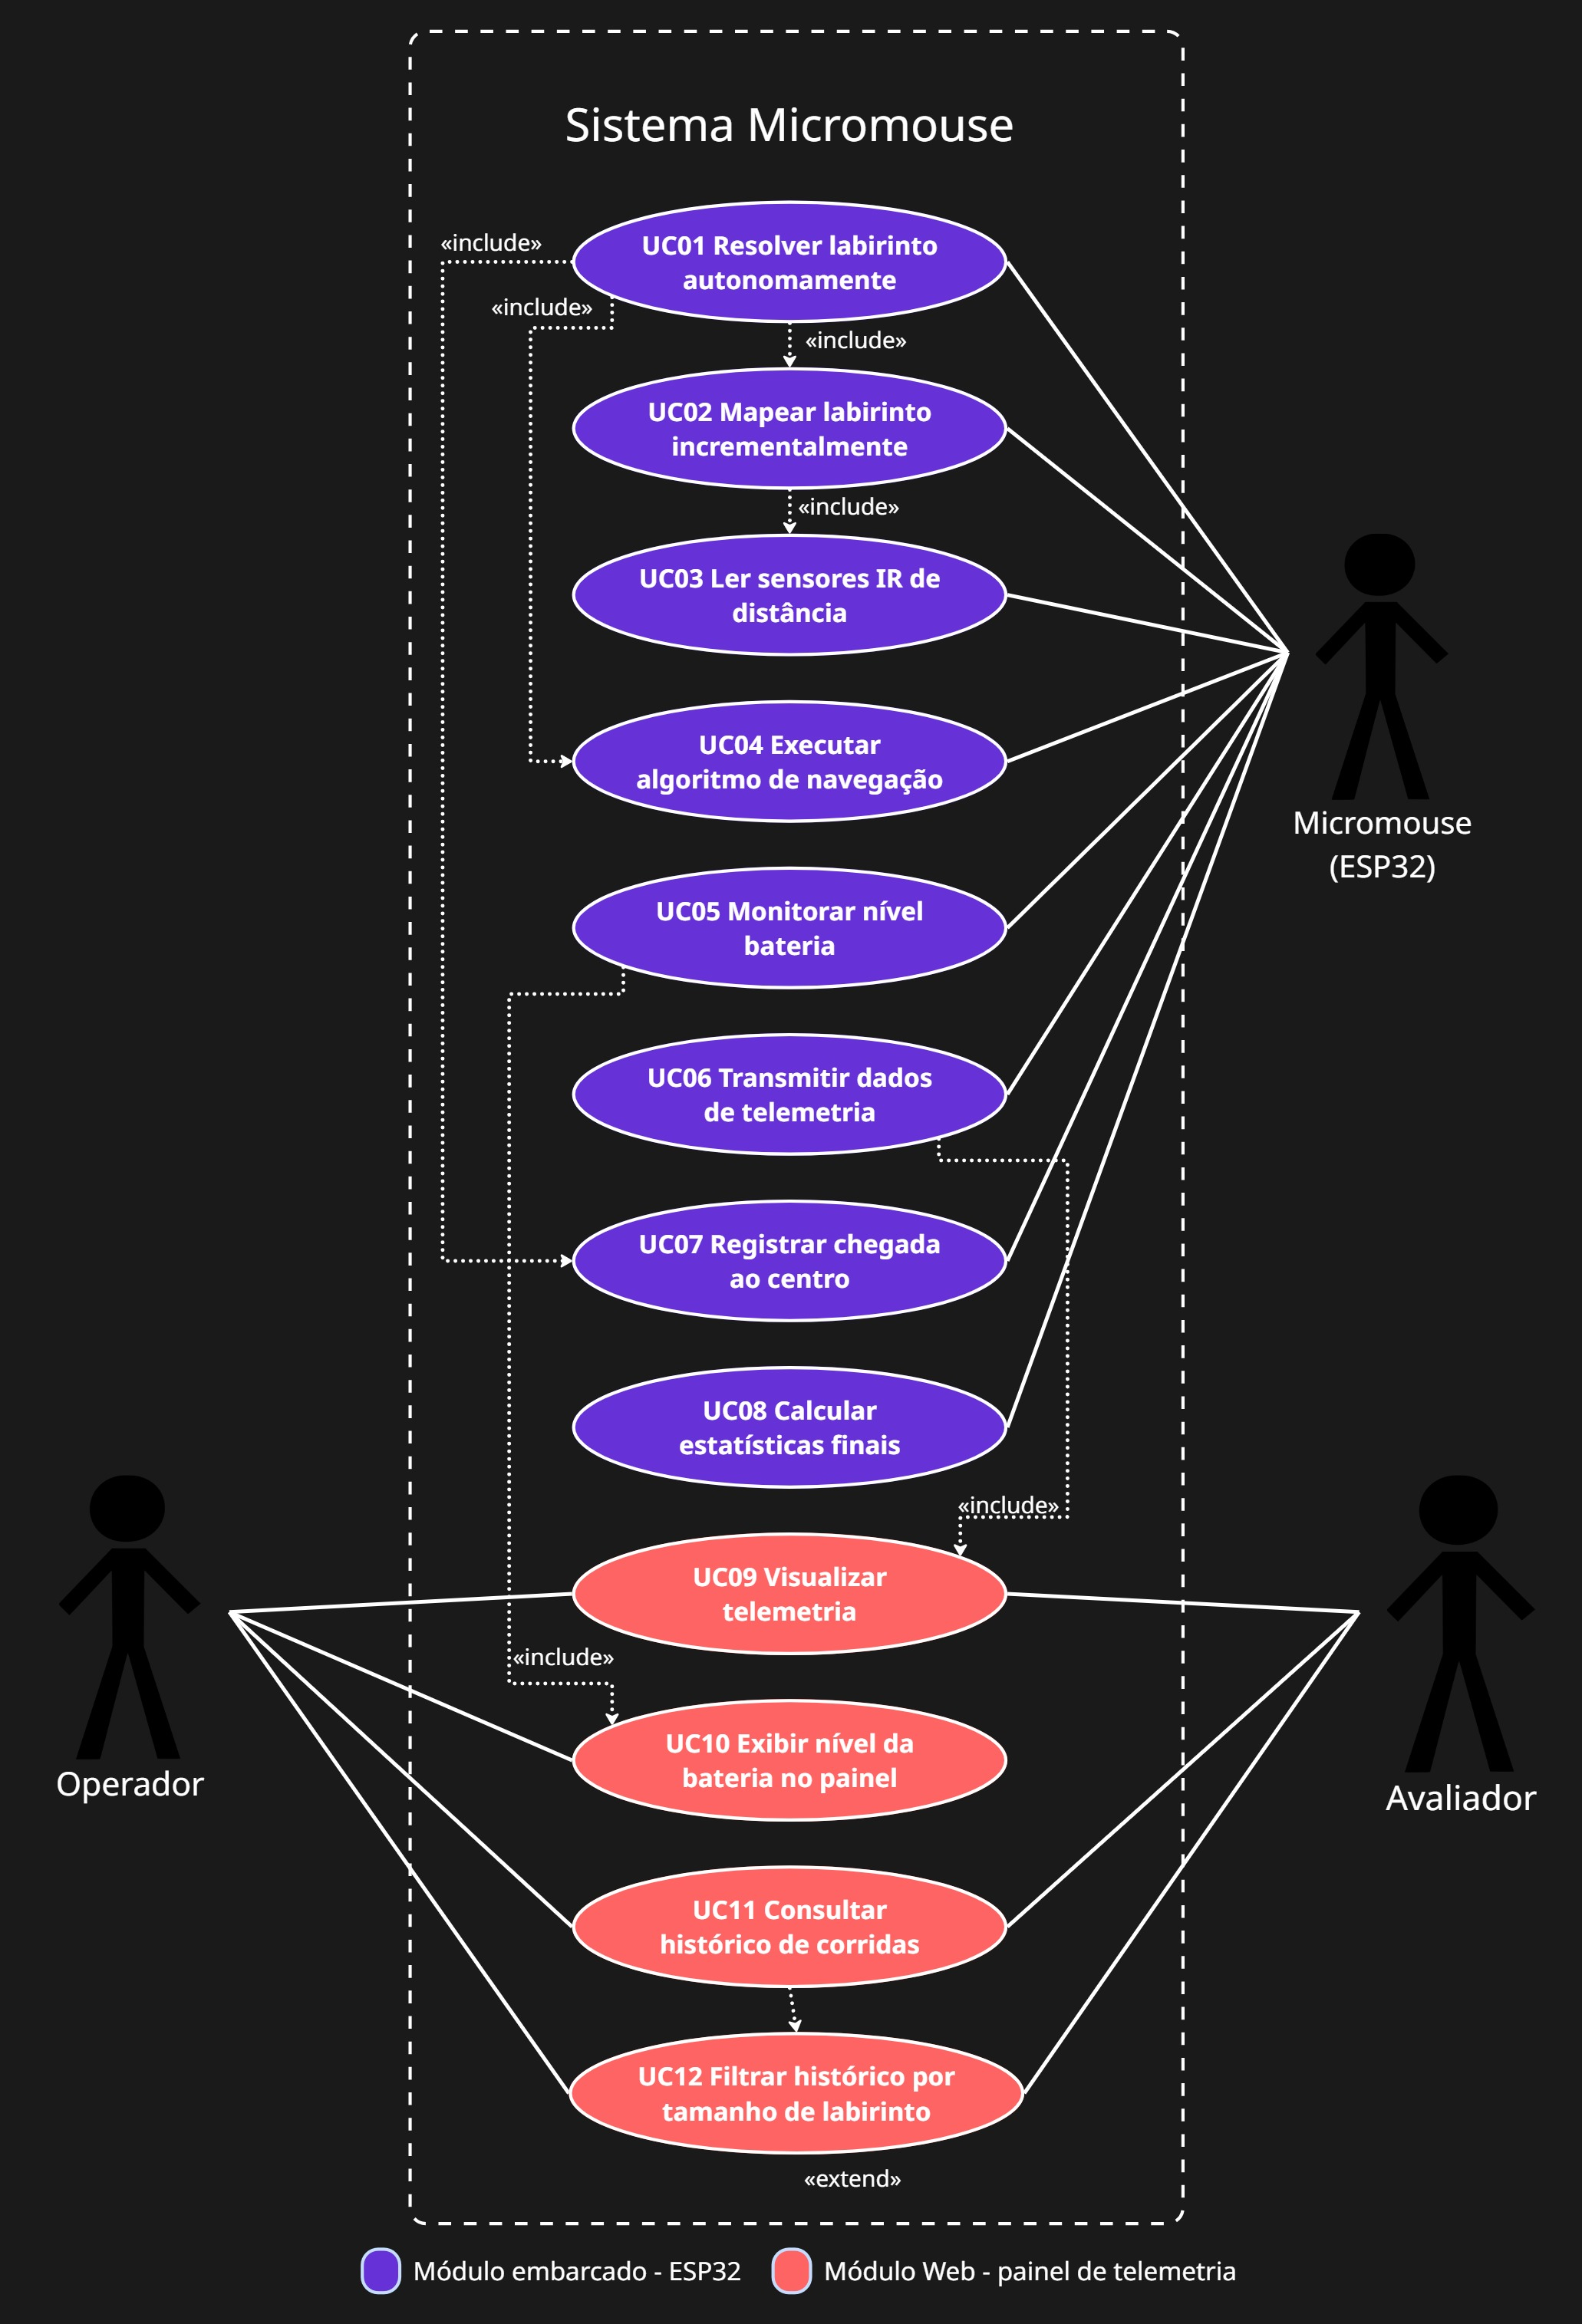
\includegraphics[
    width=0.95\textwidth,
    height=0.8\textheight,
    keepaspectratio
]{figuras/diagrama_caso_de_uso.jpg}
\captionof{figure}{Diagrama de Casos de Uso}
\label{fig:caso_de_uso_fig}
\end{center}

Os casos de uso foram agrupados por cor: em roxo os do firmware embarcado (UC01–UC08), em rosa os da plataforma web (UC09–UC12). Os três atores são o Avaliador, o Operador e o Micromouse/ESP32 (executa todos os UCs embarcados). Os relacionamentos «include» indicam dependências obrigatórias — por exemplo, UC01 sempre inclui UC02 (mapeamento). O «extend» entre UC11 e UC12 indica que filtrar por labirinto é um comportamento opcional dentro da consulta de histórico.

\paragraph{BPMN}

\begin{center}
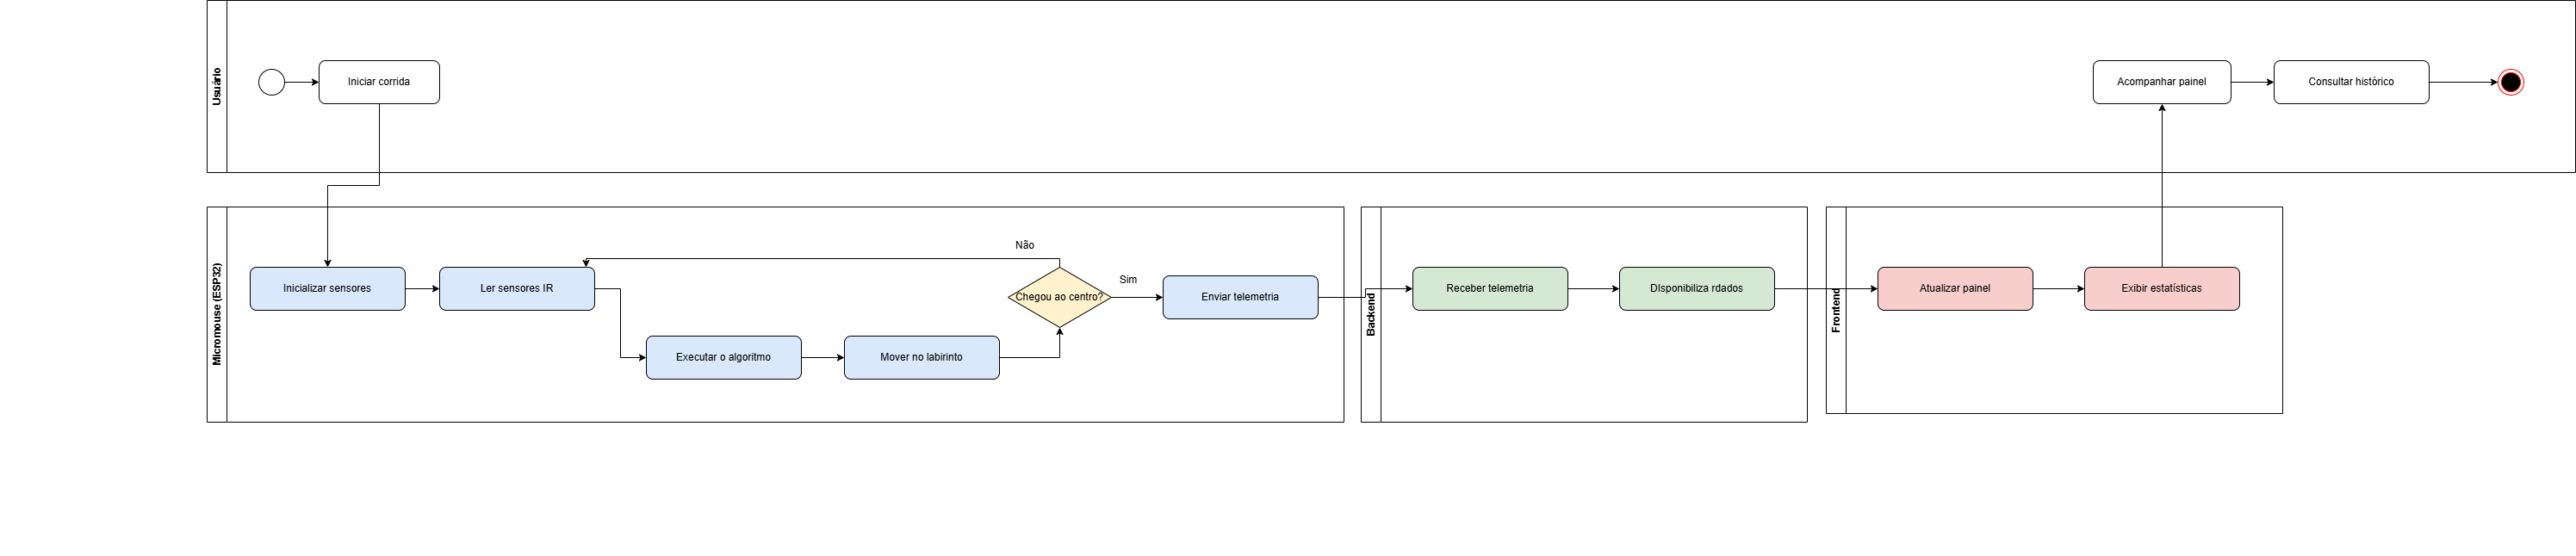
\includegraphics[
    width=0.95\textwidth,
    height=0.85\textheight,
    keepaspectratio
]{figuras/bpmn.png}

\captionof{figure}{Diagrama BPMN.}
\label{fig:bpmn_fig}
\end{center}

O diagrama BPMN representa o fluxo completo de execução do sistema Micromouse, desde o início da corrida até a visualização dos dados de telemetria. O modelo foi estruturado utilizando raias para separar as responsabilidades entre Usuário, Micromouse, Backend e Frontend.

O fluxo inicia com o operador posicionando o robô no labirinto e acionando o início da corrida. Em seguida, o Micromouse realiza a inicialização dos sensores e motores, enquanto o frontend inicia a sessão de telemetria. Após a sincronização das etapas iniciais, o robô entra no ciclo principal de exploração do labirinto.

Durante a execução, o ESP32 realiza continuamente a leitura dos sensores infravermelhos, detecta paredes, atualiza o mapa interno do labirinto e executa o algoritmo para definição do próximo movimento. Paralelamente, os dados de telemetria são enviados ao backend, incluindo posição, velocidade média, tempo de execução e nível de bateria.

O backend é responsável por processar os dados da corrida no banco de dados, enquanto o frontend web atualiza o painel de monitoramento em tempo real para o usuário. O fluxo permanece em repetição até que o robô atinja a chegada do labirinto.

Ao final da corrida, o sistema calcula as estatísticas finais, registra o resultado da tentativa e disponibiliza os dados históricos para consulta posterior através da plataforma web.

\begin{itemize}
    
    \item \textcolor{red}{ \textbf{Descrição da arquitetura da solução de \textit{software} proposta:}}
    \begin{itemize}
    
        \item \textcolor{red}{ Esta subseção deve contemplar o documento de arquitetura do sistema e deve ser estruturado segundo as visões (4+1) previstas no processo unificado (UP): lógica, de processos;  implementação, implantação e dados (substuirá a visão de casos de uso).}
        
        \item \textcolor{red}{ Propósito do \textit{software} (qual o seu papel no sistema);}
        \item \textcolor{red}{ Padrão adotado: MVC, MVP, Microsserviços, Monolítico, etc (Justificar);}
        \item \textcolor{red}{ Linguagens de programação: Java, Python, C\#, JavaScript, etc.}
        \item \textcolor{red}{ \textit{Frameworks} e bibliotecas: Spring Boot, .NET Core, React, Angular, Django, etc.}
            \item \textcolor{red}{ Banco de dados: Relacional (PostgreSQL, MySQL, etc) X NãoSQL (MongoDB,etc). }
        \item \textcolor{red}{Persistência de dados: Modelo Entidade‑Relacionamento (MER) e seu respectivo Diagrama Entidade‑Relacionamento (DER), aplicáveis quando a solução utiliza banco de dados relacional; alternativamente, diagrama de estrutura de documentos, empregado nos casos em que a arquitetura adota banco de dados não relacional.}
         \end{itemize}     
    
    \item \textcolor{red}{\textbf{ Roteiro de testes funcionais:} }
    \begin{itemize}
        \item \textcolor{red}{Código do caso de teste;}
        \item \textcolor{red}{Nome do caso de teste;}
        \item \textcolor{red}{ Objetivo do caso de teste;}
        \item \textcolor{red}{ Pré-condições do sistema para o teste ser realizado, quando se aplicar;}
        \item \textcolor{red}{ Descrição dos procedimentos a serem executados para o teste;}
        \item \textcolor{red}{ Resultado esperado para o teste ser aprovado (pós-condição após realizado o teste);}
    \end{itemize}
    \end{itemize}

